% Autor: Rami Boutassghount
% Website: https://ramiboutas.com/
% Linkedin: https://www.linkedin.com/in/ramiboutas/
% Twitter: https://twitter.com/ramiboutas
% Telegram: https://t.me/ramiboutas

\documentclass[tikz, convert={density=300}]{standalone}
\usepackage{pgfplots}
\tikzstyle{load}=[ultra thick,-latex]
\tikzstyle{stress}=[-latex]
\tikzstyle{dim}=[latex-latex]
\tikzstyle{axis}=[-latex,black!55]

\begin{document}
	\begin{tikzpicture}[cm={-1,-1,1,0,(0,0)},x=3.85mm,z=-1cm]
		\node[anchor=center,inner sep=0] at (0,-0.8,0.5)
		{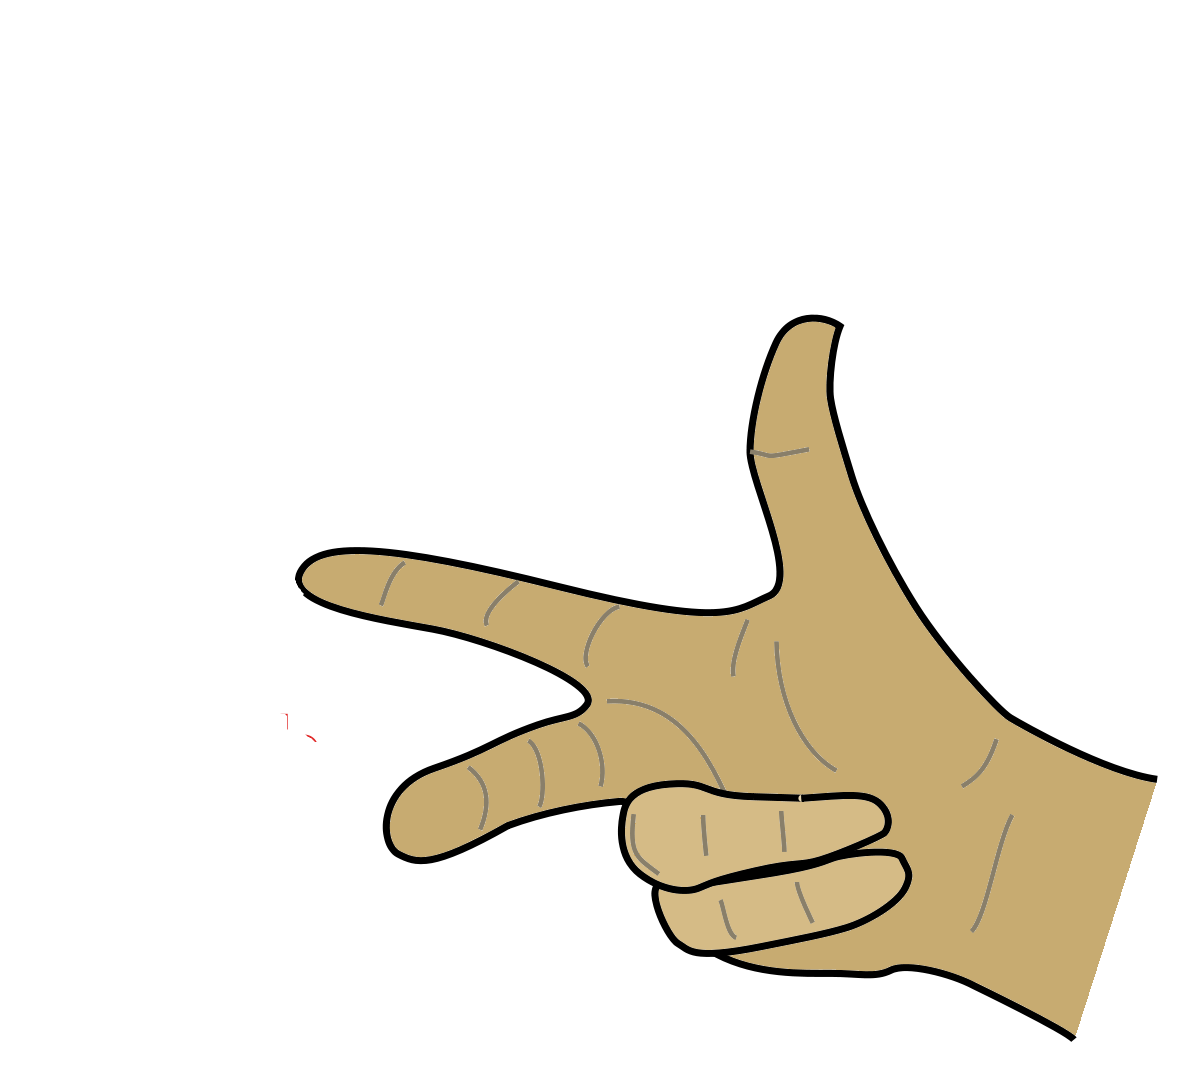
\includegraphics[width=45mm]{mano.png}};
		\coordinate (O) at (0,0,0);
		
		\def\xO{0}
		\def\yO{0}
		\def\zO{0}
		
		\def\vx{-0.3}
		\def\vy{-3}
		\def\vz{0.45}
		
		\def\wx{6}
		\def\wy{0}
		\def\wz{1.4}
		
		\def\zx{0}
		\def\zy{0}
		\def\zz{2.5}
		
		\draw[load, red] (\xO,\yO,\zO) -- ++(\vx,\vy,\vz) node[above,xshift=0.3cm] {$\vec{v}$};	
		\draw[load, blue] (\xO,\yO,\zO) -- ++(\wx,\wy,\wz) node[below,xshift=0.3cm] {$\vec{w}$};	
		\draw[load, brown] (\xO,\yO,\zO) -- ++(\zx,\zy,\zz) node[right,xshift=0.3cm] {$\vec{v} \times \vec{w}$};	
	\end{tikzpicture} 

\end{document}
